
\begin{figure}[H]
\centering
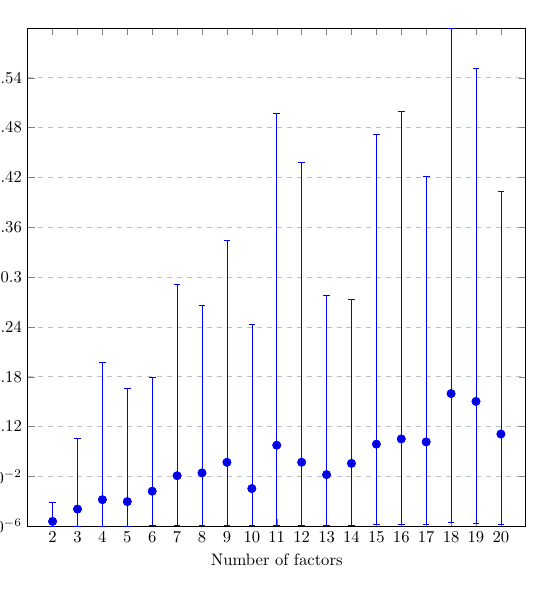
\begin{tikzpicture}[scale=0.6, trim axis left, trim axis right]
\begin{axis}[
    width=1\textwidth,
    height=1\textwidth,
    xlabel={Number of factors},
    ylabel={Time taken (s)},
    xmin=1.0, xmax=21.0,
    ymin=5e-06, ymax=0.595486,
    xticklabels={2, 3, 4, 5, 6, 7, 8, 9, 10, 11, 12, 13, 14, 15, 16, 17, 18, 19, 20},
    xtick={2, 3, 4, 5, 6, 7, 8, 9, 10, 11, 12, 13, 14, 15, 16, 17, 18, 19, 20},
    ytick={5e-06, 0.0595531, 0.1191012, 0.1786493, 0.2381974, 0.2977455, 0.3572936, 0.4168417, 0.4763898, 0.5359379},
    ymajorgrids=true,
    grid style=dashed,
]

\addplot+[
    blue,
    very thick,
    forget plot,
    only marks
    ]
    plot[
    very thick,
    error bars/.cd,
    y dir=plus,
    y explicit
    ]
    table[x=x,y=y,y error expr=\thisrow{y-max}] {
    x    y    y-max
    11	0.0967608142857	0.396752185714
10	0.0449450857143	0.196282914286
13	0.0615986857143	0.213835314286
12	0.0763987714286	0.359080228571
15	0.0980200714286	0.369938928571
14	0.0750353857143	0.195630614286
17	0.100714185714	0.317187814286
16	0.104295685714	0.391284314286
19	0.149099742857	0.398313257143
18	0.158458228571	0.437027771429
20	0.110122128571	0.289737871429
3	0.0204170571429	0.0847339428571
2	0.0057047	0.0233123
5	0.0293164285714	0.135835571429
4	0.0316512428571	0.164191757143
7	0.0603021142857	0.228674885714
6	0.0417979285714	0.135592071429
9	0.0763341	0.2652479
8	0.0636617714286	0.200044228571

    };

\addplot+[
    blue,
    very thick,
    forget plot,
    only marks
    ]
    plot[
    very thick,
    error bars/.cd,
    y dir=plus,
    y explicit
    ]
    table[x=x,y=y,y error expr=\thisrow{y-min}] {
    x    y    y-min
    11	0.0967608142857	-0.0953298142857
10	0.0449450857143	-0.0439620857143
13	0.0615986857143	-0.0603316857143
12	0.0763987714286	-0.0748697714286
15	0.0980200714286	-0.0961960714286
14	0.0750353857143	-0.0737933857143
17	0.100714185714	-0.0980221857143
16	0.104295685714	-0.102337685714
19	0.149099742857	-0.145256742857
18	0.158458228571	-0.154135228571
20	0.110122128571	-0.108252128571
3	0.0204170571429	-0.0203510571429
2	0.0057047	-0.0056997
5	0.0293164285714	-0.0289544285714
4	0.0316512428571	-0.0315432428571
7	0.0603021142857	-0.0598741142857
6	0.0417979285714	-0.0413539285714
9	0.0763341	-0.0756751
8	0.0636617714286	-0.0625907714286

    };

\end{axis}
\end{tikzpicture}
\vspace{-0.3cm}
\caption{Small primes, stop after $\sqrt{n}$ iterations}\label{fig:LenstrasEllipticCurveFactorizationsmallprimes(maximumIterations:-1)factors}
\end{figure}
